\subsection{Analysis of Calibration Frames}\label{subsec:analysis-of-calibration-frames}

The figures below show both the manual and automated calibration frame masks for
three (Figure~\ref{fig:3m_mask_overlays}) and ten (Figure~\ref{fig:10m_mask_overlays})
meters (seen in section~\ref{subsubsec:mask_creation}) superimposed atop their
corresponding raw calibration frame.

\vspace{1cm}

\begin{figure}[htbp]
    \centering
    \makebox[0.8\textwidth][c]{
        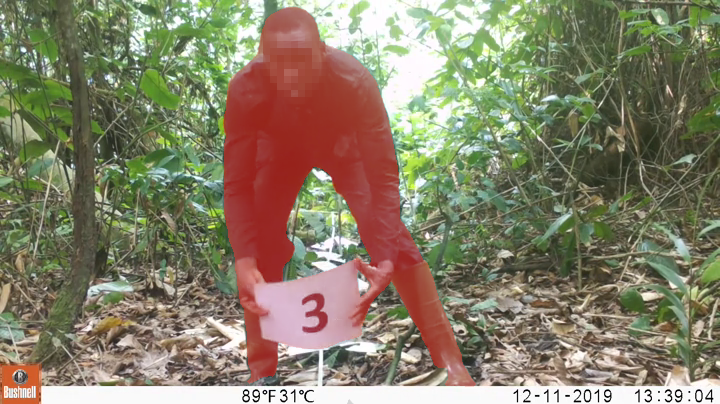
\includegraphics[width=0.9\textwidth]{body/analysis/assets/frame_masks/close_manual_overlay}
    }\\[1mm]
    \makebox[0.8\textwidth][c]{
        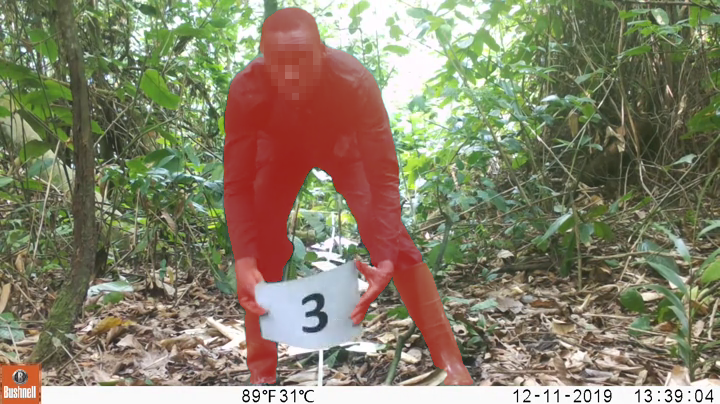
\includegraphics[width=0.9\textwidth]{body/analysis/assets/frame_masks/close_sam_overlay}
    }
    \caption{Three meter manual (top) and automated (bottom) calibration frame segmentation masks overlayed over
    the raw calibration frame}
    \label{fig:3m_mask_overlays}
\end{figure}

\begin{figure}[htbp]
    \centering
    \makebox[0.8\textwidth][c]{
        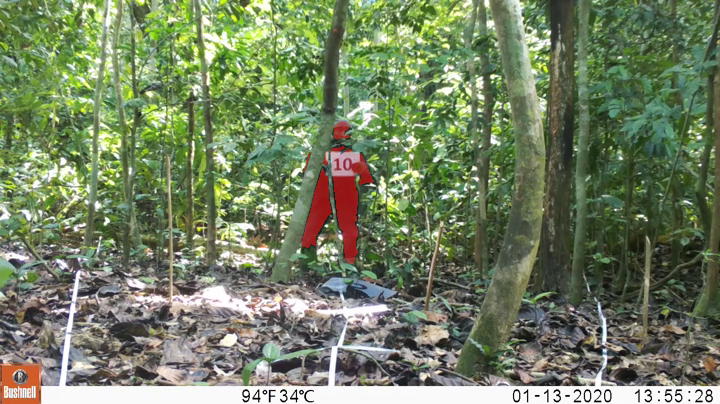
\includegraphics[width=0.9\textwidth]{body/analysis/assets/frame_masks/far_manual_overlay}
    }\\[1mm]
    \makebox[0.8\textwidth][c]{
        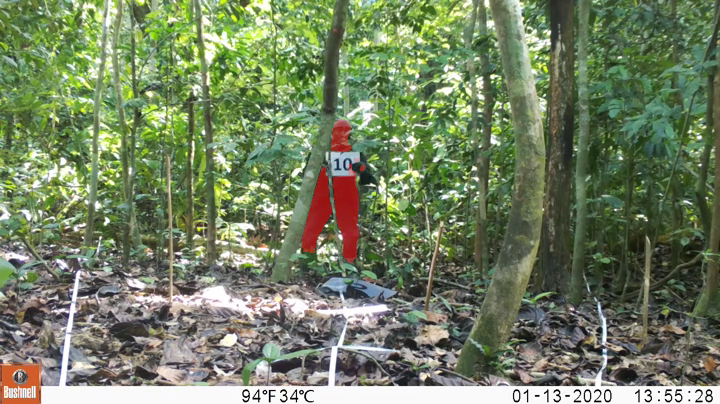
\includegraphics[width=0.9\textwidth]{body/analysis/assets/frame_masks/far_sam_overlay}
    }
    \caption{Ten meter manual (top) and automated (bottom) calibration frame segmentation masks overlayed over
    the raw calibration frame}
    \label{fig:10m_mask_overlays}
\end{figure}

\clearpage

At distances where the calibration landmark (human) is fully captured within
the frame (Figure~\ref{fig:3m_mask_overlays}), the automated approach generally yields
masks with a segmentation quality on a comparable level to those produced manually.
This pixel-perfect segmentation, however, does not hold for all calibration frames,
especially at longer distances.
For longer-distance frames (Figure~\ref{fig:10m_mask_overlays}), the landmarks occupy
fewer pixels and, most importantly, become broken up into many segments due to occlusion
from the dense foliage found in this environment.
These factors result in the loss many of the pixel-level cues that Segment Anything Model
uses to derive a segmentation boundary, leading to calibration masks that display edge-leakage
and the masking of pixels that are not themselves part of the landmark.

%\begin{figure}[htbp]
%    \centering
%    \begin{minipage}[t]{0.48\textwidth}
%        \centering
%        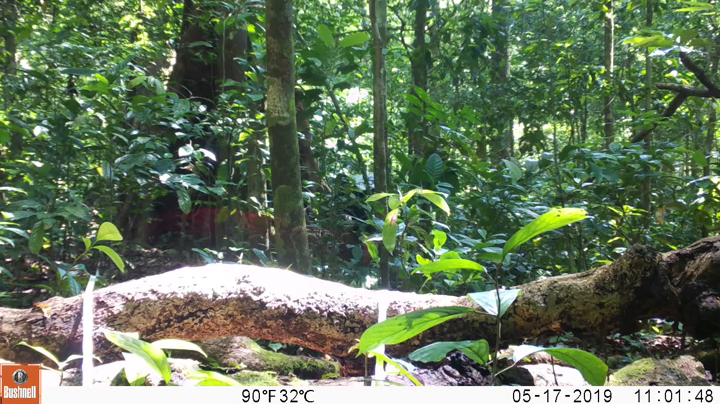
\includegraphics[width=\linewidth]{body/analysis/assets/frame_masks/15m_landmark}
%    \end{minipage}
%    \begin{minipage}[t]{0.48\textwidth}
%        \centering
%        
\includegraphics[width=\linewidth]{body/analysis/assets/frame_masks/15m_mask}
%    \end{minipage}
%
%    \caption{Calibration frame and manual binary mark corresponding to a fifteen-meter landmark)}
%    \label{fig:15m_frame}
%\end{figure}

Evident from Figures~\ref{fig:3m_mask_overlays} and~\ref{fig:10m_mask_overlays}, the
automated segmentations exclude all pixels corresponding the non-human components of the
landmarks (i.e., that distance labeled sheets of paper).
This is undesirable for the calibration process since the depth scaling of the calibration
frames should be aligned based on only the transect environment features (i.e., the pixels
outside the landmark segmentation that are common to all the calibration frames).

Additionally, calibration frames associated with the furthest of distances (i.e., approaching
fifteen meters), yielded no segmentations at all.
This is due to a failure to localise the landmarks in these frames by YOLOv5 detector.
This is an unsurprising result given the nature of the environment at the Taï National Park.
At these distances, landmark occlusion leads to extremely subtle pixel-level detection cues
and therefore great difficulty of identification even for a human.
An example of this failure case is shown in Figure~\ref{fig:15m_frame}.

\begin{figure}[htbp]
    \centering
    \makebox[0.8\textwidth][c]{
        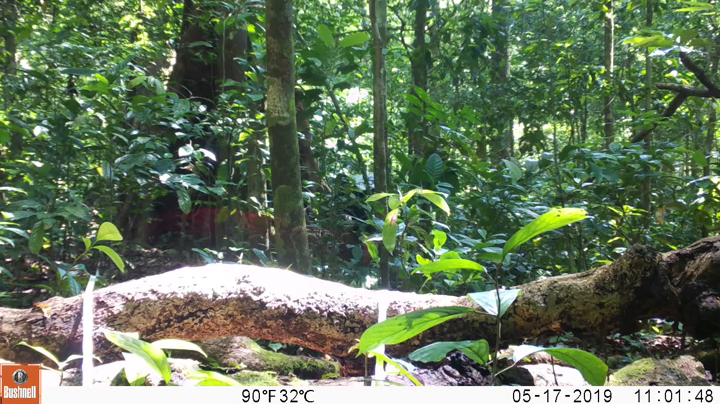
\includegraphics[width=0.9\textwidth]{body/analysis/assets/frame_masks/15m_landmark}
    }\\[1mm]
    \makebox[0.8\textwidth][c]{
        
\includegraphics[width=0.9\textwidth]{body/analysis/assets/frame_masks/15m_mask}
    }
    \caption{Example of a calibration frame (top) where landmark localisation with the automated
    masking method failed. The corresponding manual binary mark is shown on the bottom}
    \label{fig:15m_frame}
\end{figure}

Ultimately, these factors allude to the manual method of calibration frame mask creation
constituting a better approach.
Despite increased time and labour requirements, it is of greater value to achieve a
more accurate calibration than to sacrifice mask quality in order to save time during
calibration frame preparation.